Here we compare projected statistical errors of a DES-like survey 
to systematic errors introduced by shape measurement bias on 
a simulated stacked cluster weak lensing
analysis. The distribution of cluster masses that we use is 
expected to be comparable to the distribution of clusters that will
be observed by DES. The statistical error we model for the stacked
cluster mass is dominated by shape noise in the background galaxies.

To create a simulated DES-like stacked weak lensing survey we
take a halo distribution drawn according to the halo mass function \green{how do you do this? which mass function / cosmology?}. For an analysis on observed data the clusters would
be binned by observables that are correlated with cluster mass such as richness,
optical luminosity, and X-ray luminosity. Due to scatter in the observables, these bins are not strict mass bins, which however should not greatly affect the average shear profile. In this
study we divide the cluster sample into four mass bins and six
redshift bins. 


The average mass, concentration, and redshift of the
clusters in each bin is determined and then used to calculate the
expected statistical error and an average NFW shear profile.  The
number of clusters in each mass bin and their average redshift is
shown in Figure \ref{fig:N_Halo}.

To estimate the average redshift of background galaxies behind
each bin 
we use a redshift distribution of galaxies expected for a DES-like survey,
\begin{equation}
f(z) = z^m exp(-( z/z_* )^{\beta}) \; ,
\end{equation}
where $m=2.0 $, $z_*=0.5$ and $\beta = 2.0 $ as described in
\citep{obscos}. The average redshift of sources selected behind each
stacked weak lensing bin is shown in in Table
\ref{table:NWF_1_b} and Table \ref{table:NWF_4_b}.

The statistical mass uncertainty $\Delta$ ln$(M)$ for stacked weak lensing is \citep{obscos}
\begin{equation}
\Delta \rm{ln}(M) = \sqrt{ (\Delta  \rm{ln} (M_{s}))^2 +
(\sigma_{wl} )^2 } \; ,
\end{equation}
which combines the undertainty due to shape noise $(\Delta  \rm{ln} (M_{s}))$ and the scatter based on intrinsic variation in cluster shear profiles at fixed mass $(\sigma_{wl})$. From \citet{mbecker}
we take \citep[cf. also][]{ccv}
\begin{equation}
\sigma_{wl} = \frac{0.3}{\sqrt{N}}
\end{equation}
where N is the number of clusters in a given bin. To calculate the
shape noise we use the equation
\begin{equation}
\Delta \rm{ln} (M_{s}) = 6.0\times10^3
\left( \frac{N}{N_{A}} \right)^{0.5} \left( \frac{M}{M_{o}} \right)^{-0.66} \left( \frac{\overline{ngal}}{N_{o}} \right)^{-0.5}\left( \frac{D_{A}}{0.5} \right)^{-1}
\end{equation}
from \citet{obscos} \green{you need to explain the symbols in this eqn}. To model the concentration we expect
for clusters at this redshift we assign an initial concentration $c$
\begin{equation}
c= A \left(  m_{200} \over 2.0 \cdot 10^{12}  \right)^{B} \left( 1 + z_{\rm{cluster}} \right)^{C}
\end{equation}
Where  $ A = 7.85 $ ,  $ B = -0.081 $ , $ C= -0.71 $ and $m_{200}$ is
the mass within $r_{200}$ from \citep{oguri}. \green{200m or 200c? if this m-c-relation from oguri or elsewhere? the way you're citing them makes it not absolutely clear}

\begin{figure}
 \centering  % this centres figure in column
  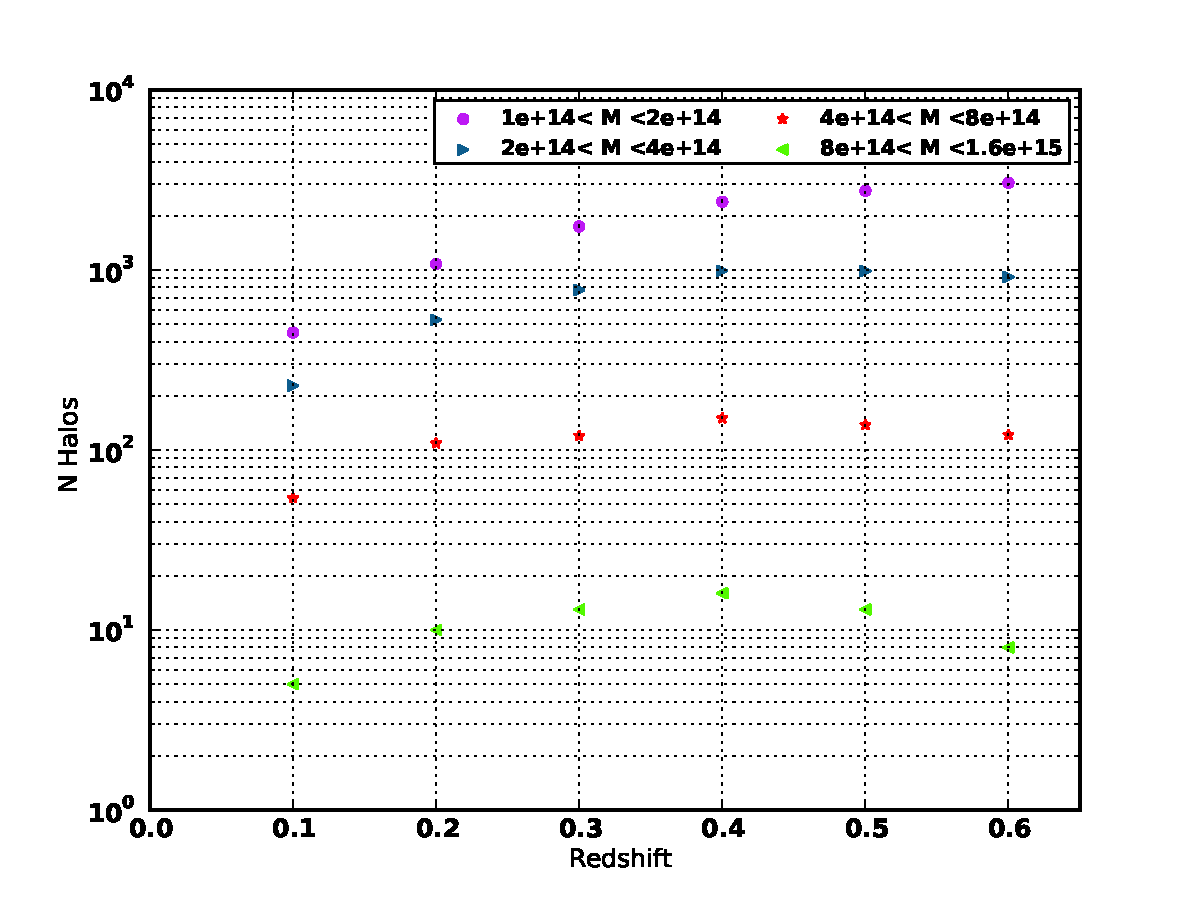
\includegraphics[width=0.55\textwidth]{fig/Halo_N.pdf} 
  \caption{The number of halos in each given mass bin.}
\label{fig:N_Halo}
\end{figure} 
